\chapter{Definición y análisis de las Fases de Exploración}
\section{Explicación general}
Durante el proceso de síntesis del controlador que realizamos mediante la exploración on-the-fly de la planta notamos que se atraviesan ciertas etapas (o fases) cuyos objetivos parciales no siempre coinciden, más allá de ser etapas que conducen a un objetivo en común (resolver el problema de control en general). La exploración atraviesa estas etapas de forma totalmente agnóstica a la heurística elegida porque están relacionadas directamente con la estructura del algoritmo de exploración dirigida.

% En el capítulo anterior concluímos que la heurística RA definida consigue buenos resultados para aproximar las mejores transiciones a explorar durante el algoritmo on-the-fly. Describimos el funcionamiento mediante el que consigue, para cada estado $e$ dentro de los estados explorados, estimar el número de pasos necesarios para alcanzar un estado marcado. De esa forma, la heurística RA posee la ventaja de representar las estructuras necesarias para su funcionamiento con una representación reducida del estado de espacios que deshecha mucha información pero conserva la suficiente para realizar la estimación mencionada.  Esta representación reducida de alguna manera nos permite abordar de forma eficiente el problema referido como \textit{explosión de estados}, en el que cae la solución Monolítica y genera complicaciones vistas en \cite{1}
% \\
% En ese sentido, entendemos que la importancia de esta heurística nos resulta particularmente útil para la etapa inicial del problema de síntesis de un \textit{Controlador}, que requiere la alcanzabilidad de un primer estado marcado.


\section{Definición de las fases de exploración}

Vamos a definir cuatro fases que creemos importantes considerar a la hora de elegir una heurística para el problema de control general. Los puntos claves que las definirán son: encontrar el primer estado marcado, cerrar un ciclo \textit{exitoso}, concluir que el ciclo encontrado previamente sea controlable y finalmente la propagación hasta el estado inicial de la condición de controlabilidad.

\subsection{Fase 1: encontrar un estado marcado}

Consideramos como parte de la \textit{Fase 1} de exploración a todas las transiciones y estados expandidos antes de realizar la primera transición cuyo destino sea un estado marcado. Tomamos esa definición porque hasta no encontrar un primer estado marcado en nuestra exploración, por definición tampoco podríamos definir estados \textit{ganadores} como \textbf{Goal} entre los explorados. En principio, nuestro enfoque realiza una exploración que parte desde un estado inicial y busca encontrar un ciclo que satisfaga la condición \textit{\textbf{canBeWinningLoop}}. Como vimos anteriormente, la condición exige que el ciclo que evaluamos contenga un estado marcado o que algún estado dentro del mismo pueda alcanzar en un paso a otro estado catalogado como \textbf{Goal}. En ese sentido definimos formalmente a la \textbf{Fase 1} de exploración como el lapso hasta que expandamos una transición hacia un estado marcado por primera vez.

\begin{figure}[h!]
    \centering
    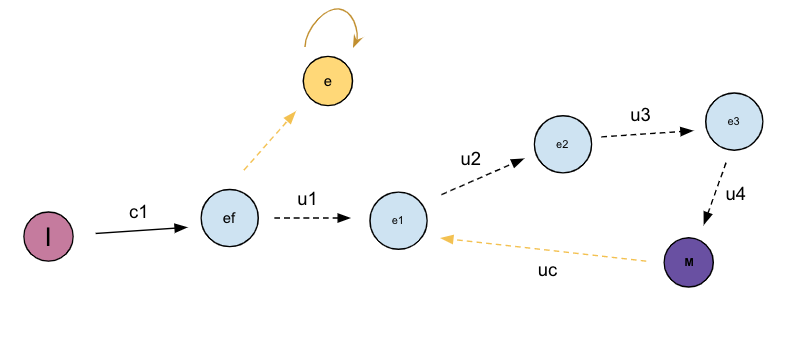
\includegraphics[width=.65\textwidth]{capitulos/cap4/img/fase1/ejemploFase1.png}
    \caption{Ejemplo de exploración que finaliza la Fase 1}
    \label{fig:fase1Ejemplo}
\end{figure}

En la figura \ref{fig:fase1Ejemplo} se puede ver como se requirieron explorar \textbf{5 estados} a través de \textbf{5 transiciones} llamadas \textit{c1, u1, u2, u3} y \textit{u4}.

% \FloatBarrier

\subsection{Fase 2: cerrando un ciclo \textit{exitoso}}

Luego de haber expandido una transición que llegue a un estado marcado y habiendo completado la \textbf{Fase 1} que fue descripta anteriormente, buscaremos que se cierre un ciclo sobre ese estado marcado que exploramos. Como podemos ver en el pseudocódigo del algoritmo principal, la función  requiere expandir una transición que cierre un ciclo dentro del total de estados explorados. Lo que buscamos será verificar formalmente la noción de cierre de ciclo. Para eso, si expandimos la transición $(e, e')$, en principio queremos chequear la siguiente condición: $\exists w \ \ldot e' \runw{w}{\structure'} e.$ \\ 
Es decir aseguramos la existencia de un camino $w$ mediante el cual alcancemos $e$ desde $e'$. En la línea siguiente vamos a conseguir, mediante la función auxiliar \textbf{getMaxLoop}, un conjunto con todos los estados que forman parte del ciclo cuya existencia aseguramos en el paso anterior. \\
Una vez que hayamos chequeado afirmativa esa condición, necesitamos hacer una segunda verificación acerca de ese ciclo en donde nos aseguramos parcialmente ciertas condiciones adicionales que en caso no cumplirse nos obligarían a descartarlo. \\
Esta segunda verificación se encuentra formalizada como función auxiliar en nuestro pseudocódigo con el nombre de \textbf{canBeWinningLoop}, función que toma un conjunto de estados que forman un ciclo y chequea la posibilidad de alguna de estas dos condiciones: que exista un estado marcado dentro de ese ciclo, o que exista algún estado dentro del ciclo evaluado que pueda alcanzar en un paso a un estado etiquetado como \textit{Goal} dentro de la exploración. En nuestro caso, como estamos ejecutando un punto del algoritmo DCS donde aún no hay estados \textit{Goals} dentro de la exploración, tendremos que verificar la primera condición. \\
En el caso de verificar exitosamente la condición expresada en la función \textbf{canBeWinningLoop} de nuestro pseudocódigo habremos encontrado un ciclo potencialmente exitoso y concluímos la \textbf{Fase 2} ejecutando, por primera vez en el algoritmo DCS, la función \textbf{findNewGoalsIn} para ese mismo ciclo.

\begin{figure}[h!]
    \centering
    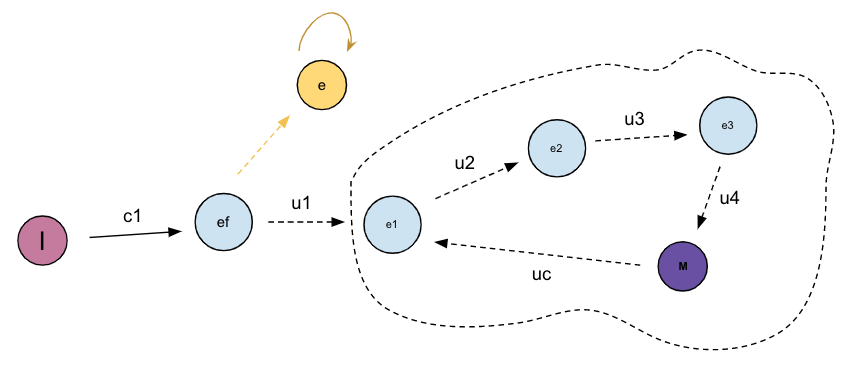
\includegraphics[width=.65\textwidth]{capitulos/cap4/img/fase2/ejemploFase2.png}
    \caption{Ejemplo de exploración que finaliza la Fase 2}
    \label{fig:fase2Ejemplo}
\end{figure}

En la figura \ref{fig:fase2Ejemplo} podemos ver que exploramos una transición adicional que no habíamos transitado en la figura \ref{fig:fase1Ejemplo}, la transición no controlable etiquetada como \textbf{uc}. Esta transición podemos ver que cierra un ciclo entre los estados \textit{e1, e2, e3 y M}, pero además es un ciclo \textit{exitoso} que garantiza la condición pedida por el método \textbf{canBeWinningLoop} ya que \textbf{M} es un estado marcado dentro del ciclo.

\subsection{Fase 3: garantizando controlabilidad del ciclo}

Esta fase comienza con la primera ejecución de la función \textbf{findNewGoalsIn} descripta en el pseudocódigo y usando como parámetro el ciclo que encontramos en la fase anterior. Esta función aplica un método de punto fijo que permite encontrar, en caso de que exista, un subciclo controlable a partir del ciclo original. Aunque los detalles y la formalización de la función están explicados en el pseudocódigo, es importante mencionar que para garantizar la \textit{controlabilidad} del ciclo se aplica iterativamente un proceso que quita algunos estados del conjunto que compone el ciclo original con cierto criterio. La idea será remover iterativamente estados que \textit{rompan} la controlabilidad del ciclo y buscar el conjunto de estados resultantes al momento en que, ante una nueva corrida, no se puedan eliminar más estados del conjunto. \\
El criterio mencionado para remover iterativamente estados del conjunto original se basa en cumplir alguna de las siguientes dos condiciones sobre cada estado $s \in C$, siendo $C$ el ciclo analizado:

\begin{enumerate}
    \item $\exists e \ldot forcedTo(s, e, \unexploredToBottom{\structure'}) \wedge e \notin (C \cup Goals)$
    \item  $\nexists s' \in C , \exists \l \ldot s' \step{\l}{\structure'} s$
\end{enumerate}
df
El punto 1 formaliza la primera razón para \textit{remover} elementos del ciclo analizado durante la ejecución de \textbf{findNewGoalsIn}. La fórmula expresa que no puede haber ningún estado dentro del ciclo que esté forzado a irse mediante una transición no controlable a un estado $e$ que no esté en el ciclo ni haya sido previamente marcado como \textit{Goal}. 

El punto 2 expresa la condición de ser un estado no alcanzable por ningún otro estado dentro del ciclo. En la primera iteración del método ningún estado cumplirá esta condición ya que el parámetro (un conjunto de estados que conforma un ciclo) conforma un grafo conexo. Una vez que empecemos a quitar elementos de este conjunto por cumplir la condición expresada en punto 1 aparecerán ciertos estados no alcanzables desde ningún otro estado del ciclo, es decir que cumplen la condición número 2.

\begin{figure}[h!]
    \centering
    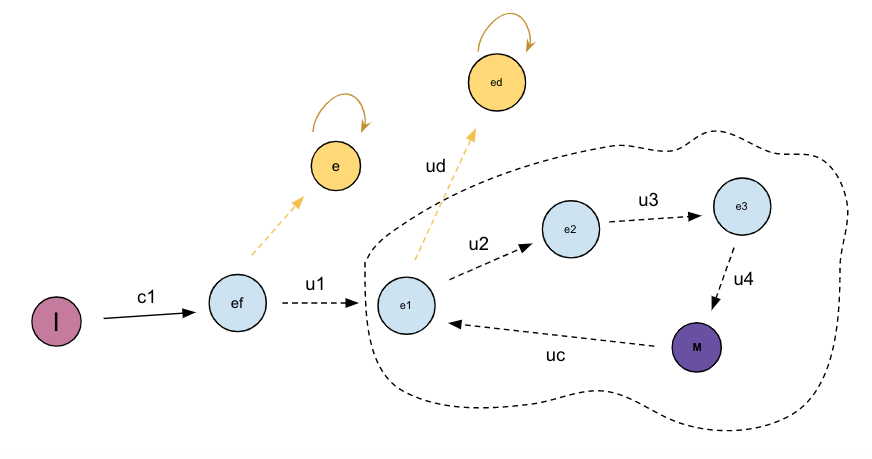
\includegraphics[width=0.65\textwidth]{capitulos/cap4/img/fase3/ejemploFTL1.png}
    \caption{Ejemplo de un ciclo (rodeado por línea de puntos)}
    \label{fig:ejemploFTL}
\end{figure}

\FloatBarrier
En la figura \ref{fig:ejemploFTL} podemos ver un ejemplo en donde la línea punteada encierra un ciclo que contiene un estado marcado y cuyos estados que lo componen serán parámetro de la función \textbf{findNewGoals}. Luego, al ejecutarse esta función y analizar los estados que componen el ciclo, encontrará que el estado \textit{e1} es un estado que cumple la primera de las condiciones que enumeramos anteriormente, ya que posee una transición no controlable \textbf{(ud)} hacia un estado $ed$ que no se encuentra dentro del ciclo ni está dentro del conjunto de estados marcados como \textit{Goal}. En ese sentido, el estado $e1$ será removido como parte de la primera iteración del método \textbf{findNewGoals}, dando lugar a una estructura reflejada en la figura \ref{fig:ejemploFTL2}. 

\begin{figure}[h!]
    \centering
    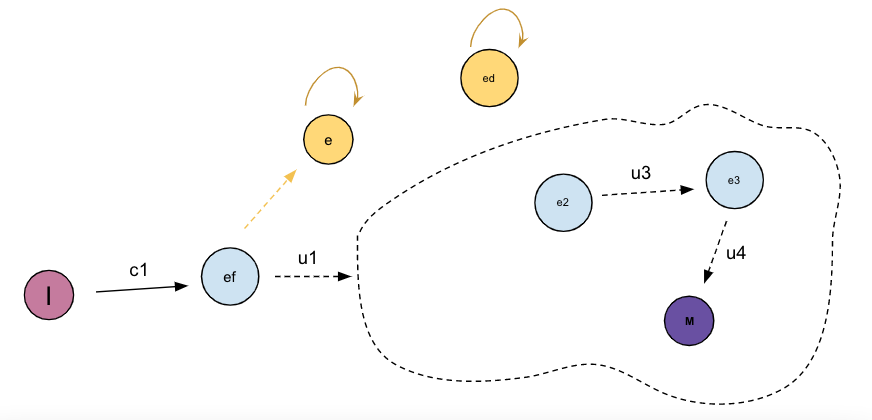
\includegraphics[width=0.65\textwidth]{capitulos/cap4/img/fase3/ejemploFTL2.png}
    \caption{Ejemplo del ciclo luego de remover en una iteración los estados del ciclo que cumplían la condición 1}
    \label{fig:ejemploFTL2}
\end{figure}

Lo que podemos ver en la figura \ref{fig:ejemploFTL2} es el conjunto resultado de la primera iteración del método \textbf{findNewGoals} luego de eliminar el estado que mencionamos anteriormente y que destacamos en la figura \ref{fig:ejemploFTL}. De esta manera destacamos al estado $e2$ que se puede ver como no cumple la condición número dos de las enumeradas previamente porque justamente se trata de un estado que, en esta iteración, ni siquiera recibe transiciones entrantes. Por lo tanto podemos determinar que no será alcanzable desde ningún estado, lo que implica que tampoco será alcanzable por un estado del ciclo.
\\
Para el ejemplo citado en las figuras, el algoritmo de punto fijo sobre el conjunto que representa al ciclo resultará con un conjunto vacío ya que todos los estados serán removidos por alguna de las condiciones comentadas previamente. Podemos ver en el pseudocódigo correspondiente a \textbf{findNewGoals} que en ese caso devolvería un conjunto vacío que no genera ningún cambio a nivel general de la ejecución del algoritmo DCS. Justamente lo que buscamos en esta fase es lograr un subciclo controlable como resultado de nuestro método, en donde exista una iteración que ya no modifique el conjunto y a la vez haya elementos que compongan el subciclo buscado. 
\\
% Acá definimos los conjuntos que se particionan en el FNG
En este sentido conviene analizar en mayor profundidad las razones por las cuales el resultado de la ejecución del método \textbf{findNewGoals} no resulta exitosa (es decir devuelve un conjunto vacío) y eso lo haremos, en principio, caracterizando algunos tipos de estados que se desprenden de la lógica del método iterativo.
\\
En principio analizaremos los estados del ciclo que es parámetro del método \textbf{findNewGoals} que cumplen con la condición de estar \textit{forzados a irse} y que formalizamos previamente. La idea de este análisis será ver que características nos permiten agrupar a esos estados. 
\\
Por un lado, nos interesa analizar los estados forzados a irse \textbf{en la primera iteración} del método \textbf{findNewGoals}. Es importante chequear esta condición en la primera iteración ya que después el método funciona quitando elementos del conjunto, por lo cual en posteriores iteraciones se pueden encontrar transiciones no exploradas por haber removido previamente al destinatario de alguna de esas transiciones. Estos estados que el método quita en la primera iteración del conjunto son los que desencadenan el resultado negativo sobre el chequeo de controlabilidad del ciclo. Podemos afirmar que, en caso de \textit{resolver} las transiciones de esos estados que \textit{lo sacan} del ciclo, hubieramos encontrado un subciclo controlable como resultado del método \textbf{findNewGoals}.

\begin{figure}[h!]
    \centering
    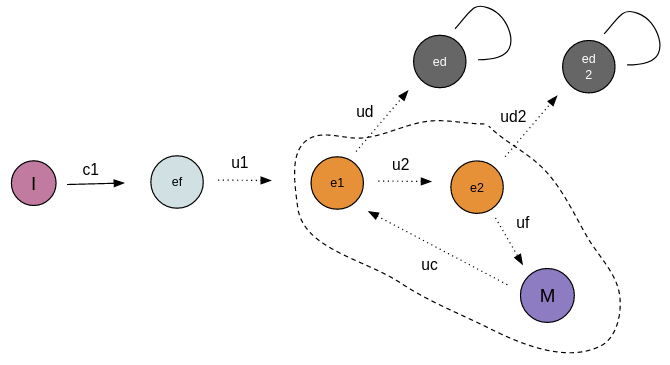
\includegraphics[width=0.65\textwidth]{capitulos/cap4/img/fase3/ejemploFTL3.png}
    \caption{Ejemplo del ciclo evaluado en la primera iteración del método FindNewGoalsIn}
    \label{fig:ejemploFTL3}
\end{figure}

En la figura \ref{fig:ejemploFTL3} y dentro del círculo punteado representamos el estado del ciclo que será evaluado en la primera iteración del método \textbf{findNewGoalsIn}. Destacamos dentro del ciclo a los estados \textbf{e1} y \textbf{e2} ya que ambos poseen transiciones no controlables \textit{(ud y ud2 respectivamente)} que conducen a estados que están por fuera del ciclo y que no están catalogados como Goal, de hecho son estados Deadlock. Queremos analizar puntualmente a los estados que cumplen esta condición ya que son claves para la resolución de esta fase de exploración. La importancia de estos estados está justificada en el hecho de suponer -para el ejemplo de la figura \ref{fig:ejemploFTL3}- que si las transiciones \textbf{ud} y \textbf{ud2} condujeran a caminos controlables que \textit{vuelvan} al ciclo entonces resolveríamos el problema de control planteado en \textbf{findNewGoalsIn}. La Fase 3 finaliza cuando el problema de controlabilidad del ciclo sea resuelto y encontremos un subciclo controlable, el cual nos servirá de parámetro para empezar la Fase 4.

\subsection{Fase 4: propagación de estados Goal}

Concluímos la fase anterior devolviendo un subciclo controlable que contiene un estado marcado. Este proceso es condición necesaria para resolver nuestro problema en general ya que nos permite lograr no solo alcanzabilidad a un estado marcado, sino también una manera de llegar de forma controlable a el. Por como fue definido el problema de control previamente, partimos la exploración desde un estado inicial desde el cual tenemos que poder alcanzar, también controlablemente, el subciclo mencionado.
\\
La Fase 4 inicia con la primera ejecución del método \textbf{propagateGoal}, cuyo parámetro será el ciclo controlable que encontramos en la fase anterior. Este método buscará garantizar que podamos llegar controlablemente desde el estado inicial hacia alguno de los estados del ciclo.
\\
Por lo tanto, primero buscaremos encontrar todos los estados \textit{ancestros} explorados que no hayan sido etiquetados como \textit{Goal} o \textit{Error} de los elementos del ciclo mediante el método \textbf{ancestorsNone}. Los \textit{ancestros} conseguidos mediante esta función se formalizan con el siguiente conjunto:

\vspace{.5cm}

\begin{center}
$\{ \, e \in \Review{\structure'} \mid \exists e' \in ciclo \ldot \exists w \ldot \trimlst{e \runw{w}{\Review{\structure'}} e'} \wedge$
          $ \nexists s \in \Review{w(e)} \ldot \Review{s \neq e' \wedge } s \in \Goals \cup \Errors \}$
\end{center}

\vspace{.5cm}

Sobre este nuevo conjunto de estados \textit{ancestros} del ciclo controlable y etiquetados como \textbf{None}, realizaremos un proceso iterativo similar al de la fase anterior en donde vamos a remover estados que cumplan con algunas de las siguientes condiciones:

\begin{itemize}
    \item Quitaremos estados que en el proceso de propagación encontremos que estén \textit{forzados a irse}. Esto quiere decir que son estados que tienen transiciones no controlables hacia elementos que no están en el ciclo ni hayan sido etiquetados como Goal previamente. 
    Estos estados se pueden describir formalmente para todos los estados $s \in ancestorsNone(estadosCiclo)$ de la siguiente manera:
    \begin{center}
        \textbf{forcedTo}($s, S_{\unexploredToBottom{\structure'}}\setminus (C \cup \Goals),\unexploredToBottom{\structure'}$)
    \end{center}
    
    \item Por otro lado también vamos a remover iterativamente los estados que no puedan alcanzar un estado \textbf{Goal} y cuya condición se describe formalmente en la siguiente línea cuya definición más extensa encontraremos en el pseudocódigo:
    \begin{center}
        $\neg$\textbf{canReachGoalIn}($s, C,\unexploredToBottom{\structure'}$)
    \end{center}

\end{itemize}

\vspace{.5cm}

\begin{figure}[h!]
    \centering
    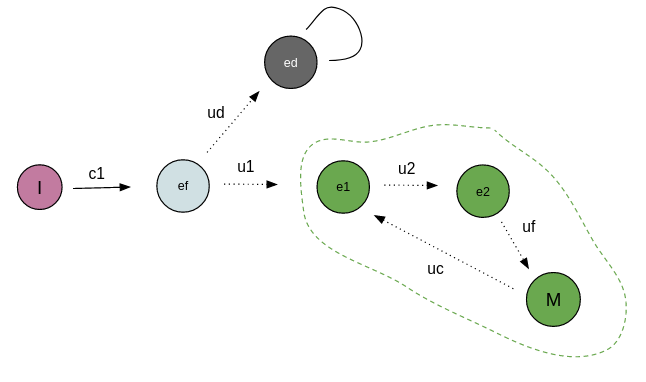
\includegraphics[width=0.7\textwidth]{capitulos/cap4/img/fase4/ejemploPropFallido.png}
    \caption{Ejemplo de proceso de PropagateGoal fallido}
    \label{fig:propGoalFallido}
\end{figure}

\FloatBarrier

En la figura \ref{fig:propGoalFallido} podemos ver un caso en donde ejecutamos el método \textbf{propagateGoal} habiendo completado la Fase 3 por encontrar un subciclo controlable con un estado marcado (marcado con línea de puntos resaltada en verde). Sin embargo, el proceso de propagación iniciado desde todos los estados del ciclo falla al llegar al estado \textit{ef}, el cual tiene una transición no controlable \textbf{ef} saliente hacia un estado \textbf{marcado como deadlock}. 
\\
En ese sentido buscamos caracterizar los estados que nos llevan a \textit{perder} en el proceso de la \textbf{Fase 4} por no lograr una propagación controlable hacia el estado inicial. Este análisis nos puede dar algunos indicios de cara a la elaboración de una estrategia que minimice las ejecuciones de \textbf{propagateGoal}. En principio no encontramos características en las heurísticas con las que venimos trabajando \textit{(Random, BFS, RA)} que utilicen esta información de cara a elegir transiciones para la exploración. Este aspecto nos motivará de cara a la siguiente sección, en la cual buscaremos variantes de las heurísticas existentes que permitan utilizar nueva información.

\begin{figure}[h!]
    \centering
    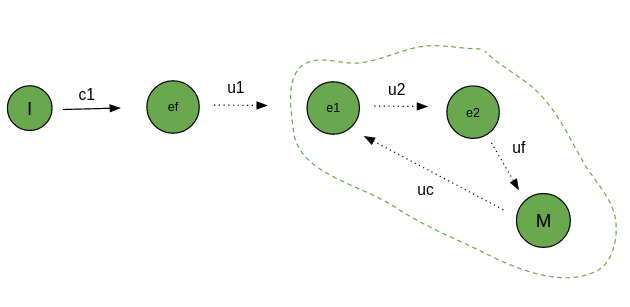
\includegraphics[width=0.7\textwidth]{capitulos/cap4/img/fase4/ejemploPropExitoso.png}
    \caption{Ejemplo de proceso de PropagateGoal exitoso}
    \label{fig:propGoalExitoso}
\end{figure}

\FloatBarrier

En la figura \ref{fig:propGoalExitoso} podemos ver en cambio un caso en donde concluye exitosamente la Fase 4. El ciclo controlable es idéntico al planteado en la figura \ref{fig:propGoalFallido}, al igual que el principio de la propagación que busca hacer esta fase. La diferencia está en haber sacado la transición no controlable etiquetada como \textit{ud} que incluíamos en la figura \ref{fig:propGoalFallido} y que convertía en no controlable el camino que recorríamos en la propagación desde el ciclo hasta el inicial.

\newpage
\section{Peso de las etapas en la exploración}
\subsection{Descripción de los casos de estudio}
En la siguiente \textit{subsección} mostramos los resultados de una experimentación que nos permitirán medir el peso relativo que tiene cada una de las etapas descriptas anteriormente en el proceso de exploración general. Decidimos usar el mismo conjunto de problemas que el utilizado para examinar la performance del algoritmo original de síntesis en \cite{DuranZanollo}. A continuación describimos brevemente todos los casos de estudios, los cuales fueron escritos con la posibilidad de ser escalados en el número de componentes y estados:

\begin{itemize}
    \item \textbf{Transfer Line:} Automatización de una fábrica, un dominio de mucho interés en el área de supervisory control. \textbf{TL} consiste de \textit{n máquinas} conectadas por n buffers cada uno con capacidad de \textit{k unidades}, termina en una máquina adicional llamada Test Unit.
    
    \item \textbf{Dinning Philosophers:} Problema clásico de concurrencia. En \textbf{DP} hay \textit{n filósofos} sentados en una mesa redonda, cada uno comparte un tenedor con sus vecinos aledaños. El objetivo del sistema es controlar el acceso a los tenedores de manera que los filósofos puedan alternar entre comer y pensar; evitando deadlock y starvation. Adicionalmente, cada filósofo, luego de tomar un tenedor, debe cumplir con \textit{k pasos de etiqueta} antes de comer.
    
    \item \textbf{Cat and Mouse:} Juego de dos jugadores donde cada uno toma turnos para moverse a una casilla adyacente dentro de un mapa de la forma de un corredor dividido en 2k + 1 áreas. En \textbf{CM} \textit{n gatos y la misma cantidad de ratones} son colocados en extremos opuestos del corredor. El objetivo es mover a los ratones de manera que no terminen en el mismo lugar que un gato. Los movimientos de los gatos no son controlables. En el centro del corredor hay un agujero que lleva a los ratones a un área segura.
    
    \item \textbf{Bidding Workflow:} Modela el proceso de evaluación de proyectos de una empresa. El proyecto debe ser aprobado por \textit{n equipos}. El objetivo es sintetizar un flujo de trabajo que intente llegar a un consenso, es decir, aprobar/rechazar el proyecto cuando todos los equipos lo aceptan/rechazan. La propuesta puede ser reasignada para reevaluación por un equipo hasta \textit{k veces}, no se puede reasignar si el equipo ya lo habı́a aceptado. Cuando un equipo \textit{lo rechaza k veces} el proyecto puede ser rechazado sin consenso. Es un caso de estudio tı́pico del dominio de Business Process Management.
    
    \item \textbf{Air-Traffic Management:} Representa la torre de control de un aeropuerto, que recibe \textit{n peticiones} de aterrizaje simultáneas. La torre necesita avisar si tiene permiso para aterrizar o, en caso contrario, en cuál de los \textit{k espacios aéreos} debe realizar maniobras de espera. El objetivo es que todos los aviones puedan aterrizar de manera segura. El problema solo tiene solución si la cantidad de aviones es menor a la de espacios aéreos (n $<$ k).
    
    \item \textbf{Travel Agency:} Modela una página on-line de ventas de paquetes de viajes. El sistema depende de \textit{n servicios} de terceros para realizar las reservas (ej. alquiler de auto, compra de pasajes, etc). Los protocolos para utilizar los servicios pueden variar de manera no controlable; una variante es la selección de hasta \textit{k atributos}(ej. destino del vuelo, clase y fechas). El objetivo del sistema es orquestar los servicios de manera de obtener un paquete de vacaciones completo de ser posible, evitando pagar por paquetes incompletos.
\end{itemize}

Por otro lado, para medir la performance del benchmark descripto utilizamos el registro de tiempo total, transiciones expandidas y estados expandidos al finalizar la exploración. Todos estos resultados los estaremos midiendo, finalmente, para dos heurísticas que nos permitan realizar una comparación exploratoria sobre su impacto en las fases. Estas dos heurísticas que guían la exploración serán Breadth First Search (BFS) y RA \cite{Ciolek}. Descartamos la utilización en este caso de una heurística Random debido al elevado numero de ejecuciones requeridas para tener resultados con estadística ya que las ejecuciones no son deterministas, y debido a que BFS y RA superan en \textit{performance} a Random (podemos verlo en \cite{DuranZanollo}, por lo cual esas heurísticas nos alcanzan como base.

\subsection{Resultados}

Sabemos que cada heurística tiene distintos pesos relativos sobre cada una de las fases comentadas como se puede ver en las tablas que figuran en el anexo de este trabajo. Para poder comparar el peso relativo de cada una contrastaremos los dos tipos de heurísticas más exitosas según el trabajo visto en \cite{Ciolek} que son RA y BFS.

En la tabla \ref{tab:estadosravsbfsporc} podemos ver, para cada caso de estudio, el porcentaje de instancias en las que la heurística RA explora menos estados que la heurística BFS. Consideramos únicamente las instancias que son resueltas por ambas heurísticas garantizando soluciones controlables al problema de síntesis.

\begin{table}[h!]
\begin{center}
\begin{tabular}{| c | c | c | c | c | c | c | }
\hline
\multicolumn{7}{ |c| }{Performance de estados explorados por fase RA vs BFS} \\ \hline
Fase / Caso & TA & AT & BW & CM & DP & TL \\ \hline
Fase 1 & 33\% & 30\% & 80\% & 100\% & 100\% & 100\%  \\
Fase 2 & 33\% & 25\% & 84\% & 100\% & 100\% & 100\%  \\
Fase 3 & 100\% & 85\% & 84\% & 100\% & 100\% & 100\% \\
Fase 4 & 100\% & 25\% & 100\% & 65\% & 100\% & 100\% \\
Total & 100\% & 85\% & 84\% & 100\% & 100\% & 100\% \\ \hline
\end{tabular}
\caption{Porcentaje de instancias que RA resuelve con menor cantidad de estados explorados que BFS por fase}
\label{tab:estadosravsbfsporc}
\end{center}
\end{table}

Los resultados que podemos ver en la tabla \ref{tab:estadosravsbfsporc} muestran que, considerando el total de estados expandidos, la heurística RA \textit{gana} sobre BFS en mas de un 84\% de las instancias analizadas para cada tipo de caso de estudio. Sin embargo, analizando por fases hay algunos casos donde RA pierde frente a BFS como podemos ver en Fase 1 y Fase 2 de TA y AT, y Fase 4 de AT.

Sin embargo, la tabla \ref{tab:estadosravsbfsporc} no nos brinda información cualitativa sobre en qué medida la heurística \textbf{RA} mejora en cantidad de estados explorados a la resolución que propone \textbf{BFS}. Para eso, proponemos analizar los datos utilizando un nuevo indicador. Definimos para una fase $f  \in \{1,2,3,4\}$ fija y dos heurísticas RA y BFS, el indicador \textbf{$I_f$} de la siguiente manera:

\vspace{1.2cm}

\[ I_f = 
\frac{\sum_{i \ \in \ Inst.} CantEstados_{RA}^{f}(i)}{
\sum_{i \ \in \ Inst.} CantEstados_{RA}^{f}(i) + 
\sum_{i \ \in \ Inst.} CantEstados_{BFS}^{f}(i)}
\]

\vspace{1.2cm}

Si consideramos que $CantEstados_{RA}^{f}(i)$ y $CantEstados_{BFS}^{f}(i)$ son funciones auxiliares que nos devuelven la cantidad de estados explorados en cada fase \textit{f} y para una instancia \textit{i} en ambas heurísticas. De esta forma, sumando y luego comparando el desempeño en el total de las instancias nos otorga una métrica con la que medimos cualitativamente \textit{cuanto mejor desempeño} tiene la heurística RA sobre BFS por fase. 

% Si expresamos este valor porcentualmente en términos del esfuerzo conjunto de ambas heurísticas para resolver una fase, una coordenada de esta tabla será el porcentaje de estados totales que usa \textbf{RA} obtuvo como desempeño en cuanto a \textbf{BFS}. 

A continuación otorgamos una descripción más precisa acerca del significado que tienen los posibles valores de este indicador y que los podemos interpretar de la siguiente manera:

{\centering
\vspace{0.7cm}

I_f \cong \left\{ \begin{array}{lcc}
            \\ 0 &  si  & \textbf{RA} \ $no explora estados en esa fase$ \\
            \\ 0 \  \textless \ I_f \ \textless \ 0.5 &  si  & \textbf{RA} \ $explora \textbf{menos} estados que \textbf{BFS} en esa fase$ \\
            \\ 0.5 &  si  & \textbf{RA} \ $explora \textbf{igual} cantidad de estados que BFS en la fase$ \\
            \\ 0.5 \  \textless \ I_f \ \textless \ 1 &  si  & \textbf{RA} \ $explora \textbf{más} estados que \textbf{BFS} en esa fase$ \\
            \\ 1 &  si  & \textbf{BFS} \ $no explora estados en esa fase$ 
            
             \end{array}
   \right.

\centering}

\vspace{0.7cm}

Luego de haber definido este nuevo indicador, veremos en la tabla \ref{tab:estadosravsbfscomparacion} los resultados de esta métrica expresada para todos los casos y diferenciada por fase. Particularmente en los casos donde \textbf{ninguna de las dos heurísticas} utilice ningún estado para resolver una fase pondremos un guión como referencia en la tabla.

\vspace{0.3cm}

% Acá la idea es poner la sumatoria de transiciones de cada fase para todas las instancias usando heurística RA sobre usar BFS.
\begin{table}[h!]
\begin{center}
\begin{tabular}{| c | c | c | c | c | c | c | }
\hline
\multicolumn{7}{ |c| }{Performance de estados explorados por fase RA vs BFS} \\ \hline
Fase / Caso & TA & AT & BW & CM & DP & TL \\ \hline
Fase 1 & 0,63 & 0,32 & 0,27 & 0,08 & 0,01 & 0,01  \\
Fase 2 & 0 & 0,007 & 0 & 0,01 & 0 & 0  \\
Fase 3 & 0,27 & 0,69 & 0,51 & 0,09 & 0,004 & 0,001 \\
Fase 4 & - & - & - & 1 & 0,06 & -  \\
Total & 0,28 & 0,42 & 0,42 & 0,2 & 0,007 & 0,006 \\ \hline
\end{tabular}
\caption{Indicador $I_f$ definido para cada caso del Benchmark y Fase definida}
\label{tab:estadosravsbfscomparacion}
\end{center}
\end{table}

\vspace{0.3cm}

En principio conviene remarcar de la tabla \ref{tab:estadosravsbfscomparacion} como \textit{RA} supera en \textit{performance} a \textit{BFS} en todos los casos obteniendo valores cercanos a cero para la etapa 2 y reduciendo los tiempos del resto de las etapas, salvando excepciones como la fase 1 de \textbf{TA} y las fases 3 de \textbf{BW} y \textbf{AT}, donde tenemos valores superiores al 0,5. Particularmente los casos \textbf{DP} y \textbf{TL} obtienen, usando \textit{RA}, resultados significativamente mejores en cada una de sus fases.

Si bien observamos que en la \textbf{fase 1} para el caso \textbf{TA} \textit{BFS} logra una mejor performance y en los casos \textbf{AT} y \textbf{BW} la ventaja de \textit{RA} no es tan significativa, nos gustaría poder ver en cual etapa hay un espacio de mejora. Si bien la tabla \ref{tab:estadosravsbfscomparacion} nos muestra la comparación de performance entre las dos heurísticas, no nos indica el costo de la fase en el total del algoritmo. Para eso analizaremos, para cada caso de estudio, el porcentaje de estados explorados por fase para la heurística RA. De esta forma tendremos una intuición acerca del peso relativo que tiene la ejecución de cada fase con determinada heurística.

% Tabla que contiene el porcentaje de cada fase para cada heurística
\begin{table}[h!]
\begin{center}
\begin{tabular}{| c | c | c | c | c | c | c | }
\hline
\multicolumn{7}{ |c| }{Porcentaje de cada fase medido mediante la acumulación de estados explorados para RA} \\ \hline
Fase / Caso & TA & AT & BW & CM & DP & TL \\ \hline
Fase 1 & 5\% & \textbf{56,3\%} & 17,5\% & 2\% & \textbf{84\%} & \textbf{93\%}  \\
Fase 2 & 0\% & 0,4\% & 0\% & 0,3\% & 0\% & 0\%  \\
Fase 3 & \textbf{95\%} & 43,3\% & \textbf{82,5\%} & 34\% & 14\% & 7\% \\
Fase 4 & 0\% & 0\% & 0\% & \textbf{63,7\%} & 2\% & 0\%  \\
Total & 100\% & 100\% & 100\% & 100\% & 100\% & 100\% \\ \hline
\end{tabular}
\caption{Porcentaje de cada fase medido en estados explorados para la heurística RA}
\label{tab:pesodefasesra}
\end{center}
\end{table}


% En \textbf{DP}, \textbf{TL} y \textbf{CM} se obtiene una gran ventaja en fase 1 y 2 para las cuales podemos ver en \cite{Ciolek} un análisis más detallado sobre como en estos casos RA hace una notoria diferencia en la \textit{performance} total. Particularmente vemos en este análisis preliminar de las fases de exploración que la heurística RA explota la ventaja de calcular la estimación de distancia hacia un estado marcado, lo que permitiría acelerar la etapa 1 con respecto a otras heurísticas. 

% Sin embargo, tanto para estos casos como para los otros tres cuya performance de la heurística \textbf{RA} es levemente inferior, podemos ver que la fase 3 es la que resulta más costosa. Si bien observamos que en la \textbf{fase 1} para el caso \textbf{TA} BFS logra una mejor performance y en los casos \textbf{AT} y \textbf{BW} la ventaja de \textbf{RA} no es tan significativa, podemos ver que hay un gran espacio de mejora en la \textbf{fase 3}. 

\FloatBarrier

En la tabla \ref{tab:pesodefasesra} encontramos, para cada caso de estudio, el porcentaje de estados explorados por fase usando la heurística RA. En la sección de \textbf{apéndice} encontraremos los gráficos en los que se mide el peso de cada etapa tanto para RA como podemos ver en la tabla, como para la heurística BFS.

La tabla  \ref{tab:pesodefasesra} nos proporciona una visión acerca de las fases más \textit{costosas} para resolver el problema de síntesis usando RA. Sin embargo, aunque este aspecto es valioso, es información que deberíamos complementar con la información anterior para buscar un nuevo indicador que nos de una idea de ventanas de mejora dentro de la experimentación realizada. Para eso planteamos una multiplicación de los valores de ambas tablas, con la idea de obtener un valor que combine ambos aspectos.

En este caso, un número alto implica que determinada combinación de fase y caso de estudio obtienen poca ventaja comparativa compitiendo contra BFS (el valor de la tabla \ref{tab:estadosravsbfscomparacion} y además eran originalmente difíciles de resolver para RA porque ocupaban gran porcentaje de los estados explorados en total (el valor en la tabla \ref{tab:pesodefasesra}).

% Tabla que contiene la multiplicación de tabla 4.2 y 4.3
\begin{table}[h!]
\begin{center}
\begin{tabular}{| c | c | c | c | c | c | c | }
\hline
\multicolumn{7}{ |c| }{Indicador de costo de las fases} \\ \hline
Fase / Caso & TA & AT & BW & CM & DP & TL \\ \hline
Fase 1 & 3,15 & 18,01 & 4,72 & 0,16 & 0,84 & 0,93  \\
Fase 2 & 0 & 0,003 & 0 & 0,003 & 0 & 0  \\
Fase 3 & \textbf{25,65} & \textbf{29,87} & \textbf{42,07} & 3,06 & 0,056 & 0,007 \\
Fase 4 & 0 & 0 & 0 & \textbf{63,70} & 0,12 & 0  \\ \hline
\end{tabular}
\caption{Multiplicación entre los valores de la tabla \ref{tab:estadosravsbfscomparacion} y la tabla \ref{tab:pesodefasesra}}
\label{tab:pesoponderado}
\end{center}
\end{table}

En la tabla \ref{tab:pesoponderado} se muestra explícitamente que la ventana de mejora para los problemas que le resultan \textit{más difíciles} (TA, AT, CM y BW) a la heurística \textbf{RA} se encuentra mayoritariamente en \textbf{fase 3} para TA, AT y BW y en \textbf{fase 4} para CM. Justamente los valores grandes en la tabla corresponden a que son problemas en donde la fase 3 era originalmente pesada de resolver para RA pero además tiene poca mejora sobre BFS (lo que corresponde a un valor de porcentaje alto en la tabla \ref{tab:estadosravsbfscomparacion}). 


Por lo tanto, podemos ver luego de estos análisis que existe una gran ventana de mejora a la heurística \textbf{RA} en su desempeño de la tercera etapa para la mayoría de los casos, sobresaliendo \textbf{TA}, \textbf{AT}, \textbf{BW} y \textbf{CM} en distinta escala.

Por último mencionamos el caso de \textbf{CM} donde podemos ver particularmente el problema de fase 4 expresado en períodos donde ejecuta repetidas veces el método \textbf{propagateGoal} sin éxito. Comparando este aspecto con los resultados obtenidos usando las heurísticas vemos que, aún logrando métricas totales parecidas, en RA se traslada el peso de la etapa 3 a la etapa 4. Esto indica que, en algunos casos particulares del problema CM, la heurística RA aporta a resolver rápido la fase 3 pero le cuesta terminar de propagar los estados Goal hasta que incluyan al inicial.

% Para empezar analizaremos el comportamiento de las fases de exploración para los casos TL y DP en donde podemos ver, para la heurística Random, como obtenemos una Fase 3 mayoritaria. Parte de esta experimentación está detallada en las figuras \ref{fig:dp_estados_random} y \ref{fig:tl_estados_random} Además de obtener las peores métricas comparando en general, este detalle indica la obvia falencia de esta heurística particularmente para cerrar ciclos controlables y exitosos en estos casos. 

% Además notamos que tanto las heurísticas BFS como RA presentan una predominancia en la Fase 1 que se puede ver expresado en las figuras \ref{fig:dp_estados_bfs} y \ref{fig:dp_estados_ra}, lo que indica que proporcionalmente estas heurísticas resuelven más rápido la controlabilidad de un ciclo ganador que el hallazgo del primer estado marcado de la exploración. En BFS se puede justificar esta demora en que la búsqueda a lo ancho puede abrir varias ramas de exploración sin mantenerse en la que nos acerque a encontrar un estado marcado. Por otro lado podemos ver en \cite{Ciolek} un análisis más detallado sobre como en estos casos RA hace una notoria diferencia en la \textit{performance} total. Particularmente vemos en este análisis preliminar de las fases de exploración que la heurística RA explota la ventaja de calcular la estimación de distancia hacia un estado marcado, lo que permitiría acelerar la etapa 1 con respecto a otras heurísticas. Sin embargo, en términos relativos vemos como resultan particularmente exitosos los casos de RA cuyas fases que requieran controlabilidad (fase 3 y fase 4) sean menores. 

% En cuanto al comportamiento de otros casos del \textit{benchmark} como BW, TA y CM se puede ver como para las tres heurísticas hay predominancia de etapa 3 en las métricas medidas como puede verse en las figuras \ref{fig:bw_estados_bfs}, \ref{fig:bw_estados_ra}, \ref{fig:bw_estados_bfs}, \ref{fig:cm_estados_bfs} y \ref{fig:bw_estados_bfs} \ref{fig:cm_estados_ra} .  Esto indica que la estructura de los problemas lleva a una deficiencia para garantizar controlabilidad del ciclo durante la exploración.

% Se puede observar que más allá del análisis de fases, estos casos son donde la heurística RA no logra una mejora significativa como en los mencionados anteriormente (TL y DP). Este resultado indica que la heurística RA no hace un aporte significativo en cuanto a resolver rápidamente el problema de las fases 3 y 4. 

% En el caso de CM podemos ver particularmente el problema de fase 4 expresado en períodos donde ejecuta repetidas veces el método \textbf{propagateGoal} sin éxito. Comparando este aspecto con los resultados obtenidos usando las heurísticas vemos que, aún logrando métricas totales parecidas, en RA se traslada el peso de la etapa 3 a la etapa 4. Esto indica que, en algunos casos particulares del problema CM, la heurística RA aporta a resolver rápido la fase 3 pero le cuesta terminar de propagar los estados Goal hasta que incluyan al inicial.


\subsection{Conclusiones}

En el análisis de resultados repasamos como el aporte de la \textbf{heurística RA} mejora la métrica del total de estados explorados para todos los casos. Sin embargo, si analizamos detalladamente, en los casos donde la mejora es menor comparativamente se puede ver que hay espacio de mejora en la fase 3 que, según el análisis que concluye en la tabla \ref{tab:pesoponderado}, es la que mayor cantidad de estados ocupa en resolver el problema en general. 

Por lo tanto sostenemos la hipótesis de la posibilidad de mejora para la tercera etapa de exploración por lo comentado anteriormente y considerando que, más allá de la estructura del problema, la heurística \textbf{RA} no utiliza información específica que lleve a resolver esa fase. 

A continuación haremos un análisis más detallado del comportamiento de la tercera etapa utilizando \textbf{RA} para encontrar elementos que nos permitan mejorar las métricas de exploración para esa fase.